\documentclass[11pt]{article}
% \usepackage{tikz}
\usepackage{amsmath}
\usepackage{listings} %For code in appendix
\lstset{
  basicstyle=\ttfamily,
  mathescape
}
\usepackage{amssymb}
\usepackage{caption}
\usepackage{float}
\usepackage{subcaption}
\usepackage{graphicx}
\usepackage{hyperref}
\usepackage{float}
\usepackage{fancyhdr}
\usepackage[ruled,vlined]{algorithm2e}
\usepackage{xcolor}
\usepackage{mathtools}
\usepackage{amstext} % for \text macro
\usepackage{array}   % for \newcolumntype macro
\newcolumntype{L}{>{$}l<{$}} % math-mode version of "l" column type
\DeclarePairedDelimiter{\ceil}{\lceil}{\rceil}

\definecolor{codegreen}{rgb}{0,0.6,0}
\definecolor{codegray}{rgb}{0.5,0.5,0.5}
\definecolor{codepurple}{rgb}{0.58,0,0.82}
\definecolor{backcolour}{rgb}{0.95,0.95,0.92}

\lstdefinestyle{mystyle}{
    backgroundcolor=\color{backcolour},
    commentstyle=\color{codegreen},
    keywordstyle=\color{magenta},
    numberstyle=\tiny\color{codegray},
    stringstyle=\color{codepurple},
    basicstyle=\ttfamily\footnotesize,
    breakatwhitespace=false,
    breaklines=true,
    captionpos=b,
    keepspaces=true,
    numbers=left,
    numbersep=5pt,
    showspaces=false,
    showstringspaces=false,
    showtabs=false,
    tabsize=2
}

\lstset{style=mystyle}


\oddsidemargin0cm
\topmargin-2cm     %I recommend adding these three lines to increase the
\textwidth16.5cm   %amount of usable space on the page (and save trees)
\textheight24cm

\newcommand{\question}[2] {\vspace{.25in} \hrule\vspace{0.5em}
\noindent{\bf #1: #2} \vspace{0.5em}
\hrule \vspace{.10in}}
\renewcommand{\part}[1] {\vspace{.10in} {\bf (#1)}}

\newcommand{\myname}{Fan Pu Zeng}
\newcommand{\myandrew}{fzeng@andrew.cmu.edu}

\setlength{\parindent}{0pt}
\setlength{\parskip}{5pt plus 1pt}

\pagestyle{fancyplain}
\lhead{\fancyplain{}{\textbf{Final Project - SAT Solver}}}      % Note the different brackets!
\rhead{\fancyplain{}{\myname\\ \myandrew}}
\chead{\fancyplain{}{15-354}}

\begin{document}

\medskip                        % Skip a "medium" amount of space
                                % (latex determines what medium is)
                                % Also try: \bigskip, \littleskip

\thispagestyle{plain}
\begin{center}                  % Center the following lines
{\Large 15-354 Final Project: SAT Solver} \\
\myname \\
\myandrew \\
\end{center}

Boolean satisfiability (SAT) solvers have played an important role in software and hardware verification, automatic test pattern generation, planning, scheduling, and solving challenging problems in algebra \cite{handbook}. This report will introduce my SAT solver, its implementation details, designs and algorithms used, some comparisons between using different heuristics for splitting and choosing of variable assignments in the unforced case, challenges faced, and future directions.

\section{SAT Solver Overview}
The SAT solver uses the classical Davis–Putnam–Logemann–Loveland (DPLL) algorithm, which is based off backtracking search. In order to speed up the search process, unit propagation (also known as boolean constraint propagation), and the usage of watchlists for ease of backtracking is also implemented. Both of these will be discussed in detail later.

\section{Project Files}
\subsection{Overview}
An overview of the project files, and how to run them is given in this section to whet the appetites of the reader.

\begin{itemize}
  \item \texttt{sat.py} This is the entry point of the project, and this is also where the DPLL algorithm is implemented  in the \texttt{SATSolver} class
  \item \texttt{loader.py} This contains the \textsf{Loader} class that loaders a \texttt{.cnf} file into our proprietary CNF format
  \item \texttt{lib.py} This contains the definitions for the classes representing various SAT objects. In particular, we have the following:
    \begin{itemize}
      \item \texttt{Variable}: This represents a base variable, i.e $x_1$.
      \item \texttt{Var}: This represents a variable in one of two states: either negated (i.e $\neg x_1)$, or not negated (i.e $x_1$). A \texttt{Var} is associated with a base \texttt{Variable}. We will use the term var in our discussion to make it clear that we are talking about vars that has the potential to be negated, instead of the base variable.
      \item \texttt{Clause}: This represents a CNF clause. We require at least two vars in each clause due to our implementation of watchlists watching 2 vars. This is an acceptable assumption since if not, we can simply duplicate the same vars that already appear. Duplicated vars are allowed. Example: $(x_1 \vee x_2 \vee \neg x_3)$
      \item \texttt{SAT}: This contains a list of CNF clauses, which represents our SAT instance. Example: $(x_1 \vee x_2 \vee \neg x_3) \wedge (\neg x_1 \vee x_2 \vee x_3)$
    \end{itemize}
  \item \texttt{assignment.py} This contains the \texttt{Assignment} class, that manages all the current variable assignment information, and also has methods related to assignments, like unit propagation and backtracking.
  \item \texttt{small/} This is a directory that contains small hand-crafted test cases that can be easily traced and verified.
  \item \texttt{Makefile} A Makefile to set up the \texttt{/dat} directory, and to run the SAT solver on each of them automatically.
\end{itemize}

\subsection{Running the SAT Solver}

To run the SAT solver, run \texttt{sat.py <filename>}. It also takes in verbosity flags, \texttt{-v} and \texttt{-vv} depending on the level desired. By default, only the test case being run and the result is given as output. \texttt{-v} prints the initial SAT formula, the current decisions being made and whenever backtracking is performed. It also outputs the final satisfying assignment. For instance, try running \texttt{./sat.py -v dat/sat/uf50-0100.cnf} to see the assignments for one of the test cases. \texttt{-vv} outputs almost all information about what the algorithm is currently doing.

As an example, try running \texttt{sat.py small/small-sat1.cnf}, which corresponds to the CNF $(x_1 \vee x_2 \vee x_3) \wedge (\neg x_1 \vee \neg x_2 \vee \neg x_3)$, which should output \texttt{SATISFIABLE}. For an unsatisfiable instance, try running \texttt{sat.py small/small-unsat2.cnf}, which is an unsatisfiable instance corresponding to the following SAT instance:
\begin{align*}
& (\neg x_1,  x_2,  x_4) \wedge
(\neg x_2,  x_3,  x_4) \wedge
( x_1, \neg x_3,   x_4)  \wedge
( x_1, \neg x_2, \neg x_4)  \wedge \\
& ( x_2, \neg x_3, \neg x_4)  \wedge
(\neg x_1,   x_3, \neg x_4)  \wedge
(  x_1,  x_2,   x_3)  \wedge
(\neg x_1, \neg x_2, \neg x_3)  
\end{align*}

This should output \texttt{UNSATISFIABLE}.

\subsection{Test Files}

The \texttt{dat} directory should already be setup in the submission directory, but in the event of issues, running \texttt{make clean} and \texttt{make setup} should restore the testcases directory (if you run into issues, please let me know - but try to avoid restoring it if there are no issues, in the event of uptime issues with the testcase source). The testcases are taken from SATLIB (\url{https://www.cs.ubc.ca/~hoos/SATLIB/benchm.html}), and are split into two folders - \texttt{dat/sat} and \texttt{dat/unsat}, for satisfiable and unsatisfiable instances respectively. Each directory contains 1000 SAT instances, each of which contains 50 variable and 218 clauses. SATLIB claims that these instances are generated uniform at random.

To run the SAT solver on all the instances that should be satisfiable, run \texttt{make sat}. This will take a while (~10 minutes). To run unsatisfiable instances, run \texttt{make unsat}. This will take even longer. This should also give a lot of confidence to the correctness of the SAT solver's implementation, as it gives the correct answers for both test suites containing 1000 test instances.

\section{Algorithm}

The two interesting algorithms implemented for SAT solving are DPLL and unit propagation. We will examine both in detail.

\subsection{DPLL}

\begin{algorithm}[H]
\SetAlgoLined
\KwResult{Either SAT or UNSAT}
  \While{not all variables assigned}{
    \If{unit propagation returns conflict}{
      \Return UNSAT
    }
    x $\leftarrow$ choose splitting var

    val $\leftarrow$ choose initial assignment for $x$

    create new decision level with $x$=val

    \While{unit propagation returns conflict}{
      \If{decision level == 0}{
        \Return UNSAT
      }
      backtrack and set splitting variable for previous decision
      level to be the negation of the original choice
    }
  }
  \Return SAT
 \caption{DPLL algorithm (implemented in \texttt{sat.py})}
\end{algorithm}

The DPLL algorithm works as follows: at every step, it chooses a variable to assign, and also chooses what value to first try assigning it. Whenever it makes such a voluntary assignment (i.e not forced), a new decision level is created \cite{katz}. A decision level contains all the current assignments, and the variable that created the decision level. In our code, this is handled by the \texttt{Assignment} class, and the \texttt{assignment\_stack} keeps track of the decision levels.

Once a new decision level is created, we perform unit propagation (elaborated next). Unit propagation forces assignments, so there is no need to create new decision levels. If unit propagation results in conflicts (i.e a clause that is unsatisfiable for sure given the current assignments), we need to backtrack. Backtracking involves returning to the previous decision level, and forcing the assignment of the variable that caused the conflicting decision level to the negation of its previous assignment. If we ever run out of decision levels, it means that all possible choices of assignments results in conflicts, and therefore the SAT instance is unsatisfiable. By using decision levels (and also watchlists, elaborated later), we can write our code in an iterative instead of recursive manner, which is significantly faster as it avoids the overhead of moving around stack frames.

In the DPLL algorithm, we allow the user to specify their own heuristics for both choosing the splitting variable, and the initial first assignment to use. This can be done by modifying \texttt{choose\_splitting\_var} and \texttt{choose\_assn} in \texttt{heuristics.py} respectively. The file is well-documented and contains information on the information that is passed in that can be used to write a useful heuristic.

By default, if either function throws \texttt{NotImplementedError}, the SAT solver will choose the first unassigned variable, and default to trying to assign it to true first. The sample implementation given in \texttt{heuristics.py} uses a randomized strategy for both \texttt{choose\_splitting\_var} and \texttt{choose\_assn}, and is meant to demonstrate how the arguments can be used.

\subsection{Unit Propagation}

The idea behind unit propagation is that when we have all other vars in a clause evaluating to false except one, then the final one must be set such that it evaluates to true. This is a forced assignment. This allows for great speedups as the search space can be drastically reduced.

Instead of naively inspecting every clause during unit propagation which is costly, we can instead only examine clauses that are actually affected by assignments \cite{swords}. In particular, we only care about clauses that contains vars whose corresponding variables are assigned a value that makes it evaluate to false. For instance, in the clause $(x_1 \vee x_2 \vee x_3)$ we can continue to sleep peacefully $x_1$ was assigned to true, but we definitely will be concerned if $x_1$ was assigned to be false.

To this end, we introduce the idea of watched literals introduced by Moskewicz et al \cite{chaff}. Each clause contains a watchlist, which contains two variables that it is currently watching. It is initialized to be the first two variables. The requirements are that we must always have at least one of the variables that it is watching be non-false (i.e either true or unknown). Whenever this is violated, the clause must find another variable to watch. If this is not possible, then unit propagation returns \texttt{CONFLICT}. 

Another benefit of using watched literals is that during backtracking, our constraints can only be relaxed (i.e our variables can be unassigned but never assigned), and therefore we do not need to update them. 

\begin{algorithm}[H]
\SetAlgoLined
\KwResult{Either OK or CONFLICT}
\textbf{propagation\_queue}: whenever we assign $x$=TRUE, we add $\neg x$ to this queue

  \While{propagation\_queue is not empty}{
    x $\leftarrow$ pop from head of \textbf{propagation\_queue}

    \For{each clause $C$ watching x}{
      y $\leftarrow$ other var watched by $C$

      \eIf{y == TRUE}{
        continue
      }{
        try to make $C$ watch a non-False var instead of x

        \If{no such var exists}{
          \eIf{y == UNKNOWN}{
            assign $y=$TRUE
          }{
            \Return CONFLICT
          }
        }
      }

    }
  }
  \Return OK
 \caption{Unit Propagation Algorithm (implemented in \texttt{assignment.py})}
\end{algorithm}

In the unit propagation algorithm given above, we go through each of the vars that is now false as a result of previous assignments, and look at all the clauses watching them, and try to maintain the invariant that each clause is watching at least one non-False variable. If this is not possible and the other variable $y$ being watched is an unknown, we then know we can force it to be true. If $y$ is already assigned, then we have a conflict, and backtracking is inevitable.

\section{Experiments with Heuristics}

The SAT solving framework provides flexibility for changing the heuristics used easily. I ran some tests to see how well they performed relative to each other, with three different strategies:

\begin{enumerate}
  \item Default strategy: use first unassigned variable, and always assign True first
  \item Randomized strategy: use any unassigned variable, and use random initial truth values
  \item Majority strategy: use first unassigned variable, and assign it the value that will satisfy the majority of the clauses that it appears in
\end{enumerate}

The results are given in the table:

\begin{tabular}{ |p{3cm}||p{3cm}|p{3cm}|  }
 \hline
 \multicolumn{3}{|c|}{Duration to run complete test suite} \\
 \hline
 \textbf{Heuristic}& \textbf{SAT}& \textbf{UNSAT}\\
 \hline
 Default & 337.15 & 795.01\\
 Random & 497.92  & 1255.64\\
 Majority & 338.17 & 810.15 \\
 \hline
\end{tabular}

\begin{figure}[t]
\centering
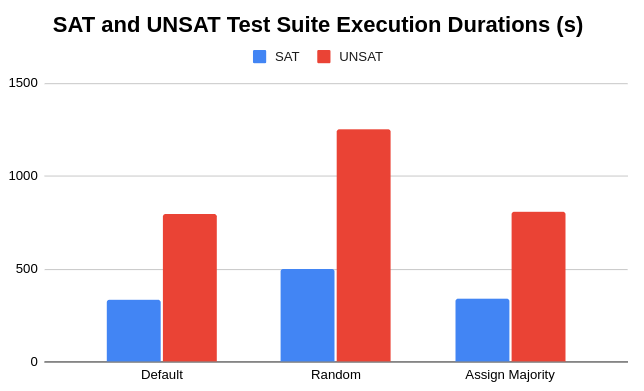
\includegraphics[width=12cm]{res}
\caption{Chart of results}
\label{res}
\end{figure}

\medskip

Figure \ref{res} shows the results graphically. It is surprising that the random strategy produces much worse results than the default strategy and the majority strategy. It is also surprising that the default naive strategy actually performs the best in this case, even though intuitively the majority strategy should perform better. A possible explanation for this behavior is that the majority strategy is a greedy strategy, and therefore random SAT instances can be resistant to greedy strategies.

\section{Challenges Faced}

Writing the SAT sovler was a fun adventure. 
Maintaining the watched literals for each clause correctly was much trickier than I expected, and I had to write a few debugging routines and put assertions to diagnose and fix a few bugs (see \texttt{check\_invariants} in \texttt{sat.py}. I also faced an insidious bug where I was modifying the watchlist of a clause while iterating through it, resulting in expected behavior. Debugging was also challenging because the SAT solver always performed correctly on my small hand-crafted SAT instances, and only failed on the much larger testcases from SATLIB which is far more difficult to trace.

It also took me a while to convince myself of the correctness of the algorithm from the interplay between the propagation queue, the watched literals, and the decision levels, although it seems completely obvious to me now.

\section{Future Directions}

There are many other promising optimizations that can be added to improve the speed of this SAT solver. 

One possibility is to implement conflict-driven clause learning (CDCL)introduced by Marques et al \cite{handbook_sat}, which is an extension of DPLL where it remembers conflicts that occurred previously and uses that to learn new clauses. This helps to prune the search space. We can also consider extending CDCL with random restarts, which has shown good results in practice \cite{restarts}. Random restarts has been shown to allow CDCL to learn about persistently troublesome conflicting variables earlier, and therefore converges to a solution faster.

Another direction is to improve our heuristics for choosing variables and their values. MOMS (Maximum Occurence in clauses of Minimum Size) is a heuristic where we prioritize assigning variables that occurs the highest number of times in short clauses. Bohm's heuristic chooses the variable that appears the most in unsatisfied clauses. The VSIDS (Variable State Independent Decaying Sum) heuristic assigns each variable a weight, which is decayed at each time step. The weight of a variable is increased whenever it is involved in a conflicting clause. The heuristic then selects the variable with the highest score.

Other directions include using conflict-directed backjumping \cite{backtrace}, which allows the solver to go more than one level up the decision level given certain conditions. Backjumping is a general technique used to speed up backtracking algorithms. 




\newpage

%Sets the bibliography style to UNSRT and imports the 
%bibliography file "samples.bib".
\bibliographystyle{unsrt}
\bibliography{references}

\end{document}
